\documentclass[a4paper, 11pt, french]{article}

\usepackage[utf8]{inputenc} 
\usepackage[T1]{fontenc}
\usepackage{geometry}
\usepackage{enumitem}
\usepackage{amssymb}
\usepackage{mathtools}
\usepackage{amsmath}
\usepackage{amsfonts}
\usepackage{varioref}
\usepackage{graphicx}
\usepackage{gensymb}
\usepackage{xcolor}
\usepackage{systeme}
\usepackage{tikz}
\usepackage[straightvoltages]{circuitikz}
\usepackage{mathrsfs}
\usepackage{esvect}

\newcommand{\R}{\mathbb{R}}
\newcommand{\C}{\mathbb{C}}
\newcommand{\N}{\mathbb{N}}
\newcommand{\Z}{\mathbb{Z}}
\newcommand{\K}{\mathbb{K}}
\newcommand{\Q}{\mathbb{Q}}
\newcommand{\p}{\wedge}
\newcommand{\D}{\mathcal{D}}
\newcommand{\dx}{\mathrm{d}x}
\newcommand{\dt}{\mathrm{d}t}
\newcommand{\tr}{\mathrm{tr}}
\newcommand{\ev}{espace vectoriel}
\newcommand{\eve}{espace vectoriel euclidien}
\newcommand{\sce}{système complet d'évènements}
\newcommand{\al}{\alpha}
\newcommand{\be}{\beta}
\newcommand{\De}{\Delta}
\newcommand{\de}{\delta}
\newcommand{\la}{\lambda}
\newcommand{\te}{\theta}
\newcommand{\si}{\sigma}
\newcommand{\Om}{\Omega}
\newcommand{\om}{\omega}
\newcommand{\ph}{\varphi}
\newcommand{\ep}{\varepsilon}
\newcommand{\som}[2]{\overset{#2}{\underset{#1}{\sum}}}
\newcommand{\produit}[2]{\overset{#2}{\underset{#1}{\prod}}}
\newcommand{\thm}{\textcolor{red}{\underline{Théorème} }}
\newcommand{\ppt}{\textcolor{red}{\underline{Propriété :} }}
\newcommand{\limit}[1]{\underset{#1}{\rightarrow}}
\newcommand{\eq}[1]{\underset{#1}{\sim}}
\newcommand{\inv}[1]{\frac{1}{#1}}
\newcommand{\acc}[1]{\left\{ #1 \right\}}


\title{Physique-Chimie MPSI}
\author{Maillet Nathan\\MP*}
\date{}

\begin{document}
	\maketitle
	N.B. : Ces exercices sont des compléments au cahier de vacance de M. Chenel
	\section*{Mécanique}
	\subparagraph*{Suspension de voiture \\} 
		On étudie le mouvement vertical du châssis d'un véhicule, par rapport aux roues. On suppose que les roues du véhicule restent en permanence en contact avec la route. Le système de suspension du véhicule peut être modélisé par l'association d'un ressort, de constante de raideur $k$, de longueur à vide $l_0$ et d'un amortisseur provoquant une force de frottement fluide $\vv{f}=-\la \vv{v}$. Pour que l'amortissement soit optimal, il faut que le châssis revienne le plus rapidement possible à sa position d'équilibre sans oscillations. On note $\vv{g}=-g\vv{u_z}$ le champ de pesanteur, où $u_z$ est le vecteur unitaire vertical orienté vers le haut. Le châssis de masse m est repéré par sa position $z$ par rapport aux roues. A l'instant $t=0$, le véhicule rencontre un trou de profondeur $h$.
	Déterminer l'expression de $z(t)$ dans le cadre d'un amortissement optimal en fonction de $z_{eq},\om_0$ et $h$ que l'on estimera grâce à $z_{eq}$ et en prenant $k=5*10^4$ kg.s$^{-2}$.

	\subparagraph*{Pyramide de Khéops \\}
		La théorie la plus couramment admise pour expliquer la construction de la pyramide de Khéops est basée sur l'utilisation d'une rampe extérieure, enduite de boues humides. Cette rampe, d'une longueur $L=600$m, et faisant un angle $\al=4.5^{\circ}$ avec l'horizontal, aurait permis d'acheminer des blocs de pierre de masse $m=2.5$t. On suppose que les ouvriers tirent le bloc de pierre avec une corde parallèle à la rampe. La norme de la réaction tangentielle de la rampe sur la pierre s'écrit : $R_T=fR_N$ où $R_N$ est la norme de la réaction normale et $f=0.1$ le coefficient de frottement dynamique. \\
Sachant que la puissance maximale fournie par un sportif de haut niveau sur une longue durée est de l'orde de $200$ W, estimer la durée nécessaire à quatre ouvriers pour monter un bloc en haut de la rampe.


	Réponse : $58$min.

	\subparagraph*{Accélérateur linéaire \\}
		Dans un accélérateur linéaire, des particules chargées de charge $q$ et de masse $m$, avec une vitesse initiale négligeable, sont accélérées entre des électrodes successives, dont la polarité est périodiquement inversée par une tension sinusoïdale d'amplitude crête à crête $U_{cc}$ et de fréquence $f$. Etablir l'expression de la longueur $L_n$ de la $n$-ième électrode.


	Réponse : $L_n=\inv{2f}\sqrt{\frac{2nqU_{cc}}{m}}$

	\subparagraph*{Chute d'un arbre \\}
		Un arbre de masse $m$ et de hauteur $h$ est coupé à sa base. A l'instant $t=0$, l'abre commence sa chute sans vitesse initiale, à partir d'un angle $\theta_0$ par rapport à la verticale. Le moment d'inertie d'une tige de longueur $h$ par rapport à l'une de ses extrémités vaut $J=\frac{mh^2}{3}$. \\
Etablir l'expression du temps de chute $\tau$ en fonction de l'intégrale $I(\theta_0)$ définie par : $$I(\theta_0)=\int_{\theta_0}^{\frac{\pi}{2}}\frac{d\theta}{\sqrt{\cos(\theta_0)-\cos(\theta)}}$$


	Réponse : $\tau=\sqrt{\frac{h}{3g}}I(\theta_0)$


	\section*{Optique}
	\subparagraph*{Distance hyperfocale \\}
		En photographie, la distance hyperfocale peut être définie comme la distance à l'objectif $h_1$ au delà de laquelle tout les objets sont nets, pour une mise au point à l'infini. On note $f'$ la distance focale de l'objectif, $D$ le diamètre d'ouverture et $c$ la taille d'une cellule élémentaire du capteur. A partir de l'expression de la distance hyperfocale, dire comment varie la profondeur de champs avec $f'$ et $D$ ? La distance hyperfocale peut également être définie comme la distance minimale $h_2$, à laquelle il est possible de faire la mise au point tout en gardant nets les objets situés à l'infini. Que peut-on dire de $h_1$ et $h_2$ lorsque $c \ll D$ ?


	Réponse : $h_1=\frac{f'D}{c}$ et $h_2=f' \left( \frac{D}{c}+1 \right) \simeq f'\frac{D}{c}$

	\subparagraph*{Modèle de Bohr de l'atome d'hydrogène \\}
		On considère un atome d'hydrogène d'un proton supposé fixe en $O$ et d'un électron animé d'un mouvement circulaire autour du proton. Montrer que le rayon de la trajectoire s'écrit $r_n=n^2a_0$ et déterminer les longueurs d'onde des raies de Balmer correspondant aux transitions entre le premier état excité $n=2$ et un état d'énergie supérieure. On donne la constante électrique $\ep_0=8.885*10^{-12}$F.m$^{-1}$.

	\section*{Thermodynamique}
	\subparagraph*{Evaporation \\}
		Dans une buanderie, de dimensions 3m sur 4m sur 2.5m, dont la température est maintenue à 27$^{\circ}$C, se trouve une flaque d'eau. L'humidité relative de l'air, définie comme le rapport de la pression partielle de l'eau sur la pression de vapeur saturante, est initialement $40\%$. La pression de vapeur saturante de l'eau à 27$^{\circ}$C est $P_s=40$mbar.


Déterminer le volume de la flaque et l'humidité relative à l'état final pour une flaque de volume initial $0.18$L et $1.8$L.

	\subparagraph*{Freinage d'urgence \\}
		Une voiture roule à $90$km.h$^{-1}$. Le conducteur freine brutalement jusqu'à s'arrêter. Les freins d'une voiture sont principalement constitués de $4$ disques d'acier de $12$cm de rayon. La capacité thermique de l'acier est de $500$J.K$^{-1}$.kg$^{-1}$ et la masse volumique de l'acier est de $800$kg.m$^{-3}$. Estimer la température atteinte par les disques de frein lors du freinage.


	Réponse : $\sim 470^{\circ}$C. 

	\section*{Électricité}
		Note : Pour les générateurs de Thevenin et l'utilisation des lois de Kirkoff et symétries, se référer aux exercices de Mr Chenel.

	\section*{Induction}
	\subparagraph*{Mesure d'une inductance mutuelle \\}
		Le montage ci-dessous permet de mesurer le coefficient d'inducante mutuelle entre deux bobines. Les deux bobines se font face comme sur la figure. La première bobine est montée en série avec une résistance $R=100\ohm$ et un générateur de tension $e_0$ harmonique de fréquence $f=5.0$kHz. Les tensions $u_1$ et $u_2$ sont mesurées grâce à un oscilloscope supposé idéal. Etablir l'expression de $u_2$ en fonction de $M,R$ et $u_1$.
\begin{figure}[h]
  \centering
  \begin{circuitikz}
    \draw (0,3) to[vsource, v_<=$e_0$] (0,0) to[short] (4,0) to[L=$L_1$] (4,3) to[generic=$R$, v=$u_1(t)$] (0,3);
    \draw (7,3) to[short] ++(-2,0) to[L=$L_2$] ++(0,-3) to[short] ++(2,0);
    \draw[->, >=latex] (7,0.5) -- node[midway, right]{$u_2(t)$} (7,2.5);
    \draw[<->] (4,3.1) to[bend left=60] node[midway, above]{$M$} (5,3.1);
  \end{circuitikz}
\end{figure}


	\subparagraph*{Freinage par induction \\}
		Deux cadres rectangulaires $\mathscr{C}_{1}$ et $\mathscr{C}_{2}$, identiques et solidaires, dont les plans forment un angle droit, sont en liaison pivot parfaite autour d'un axe $O_z$. Il n'y a pas de contact électrique entre les deux cadres. Chaque cadre a une résistance totale $R$ et une inductance propre négligeable.
Le dispositif est placé dans un champ magnétique $\vv{B}=B\vv{u_x}$.
A l'instant $t=0$, les cadres sont lancés avec une vitesse angulaire $\om_0$, depuis la position $\theta=0$. Etablir la loi $\om(t)$ et faire un bilan d'énergie entre $t=0$ et $t\limit{}+\infty$

\begin{figure}[h]
  \centering
  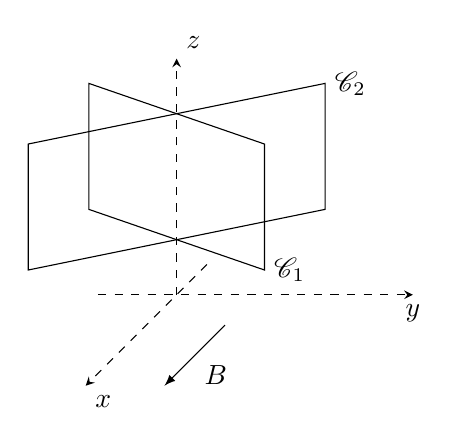
\begin{tikzpicture}
    \draw[dashed, ->, >=stealth] (0,0,-1) -- (0,0,3) node[below right]{$x$};
    \draw[dashed, ->, >=stealth] (-1,0,0) -- (3,0,0) node[below]{$y$};
    \draw[dashed, ->, >=stealth] (0,0,0) -- (0,3,0) node[above right]{$z$};
    \draw (1.5,0.7,1)node[right]{$\mathscr C_1$} -- (1.5,2.3,1) -- (-1.5,2.3,-1) -- (-1.5,0.7,-1) -- cycle;
    \draw (1.5,0.7,-1) -- (1.5,2.3,-1)node[right]{$\mathscr C_2$} -- (-1.5,2.3,1) -- (-1.5,0.7,1) -- cycle;
    \draw[->, >=latex] (1,0,1) -- node[below right]{$\vv{B}$} ++(0,0,2);
  \end{tikzpicture}
  \begin{tikzpicture}[scale=0.6]
    \draw[dashed, ->, >=stealth] (0,-4) -- ++(0,8) node[left]{$y$};
    \draw[dashed, ->, >=stealth] (-4,0) -- ++(8,0) node[right]{$x$};
    \draw (-3,-3) -- ++(6,6) node[above]{$\mathscr{C}_1$};
    \draw (-3,3) node[above]{$\mathscr{C}_2$} -- ++(6,-6);
    \draw[->, >=latex] (0,0) -- ++(1.5,0) node[below right]{$\vv B$};
  \end{tikzpicture}
\end{figure}

	\section*{Atomistique}
		Note : Pour l'atomistique, se référer aux exercices de M. Chenel.

	\section*{Transformations chimiques}
		\subparagraph{Suivi manométrique \\}
	Le butadiène est utilisé dans la synthèse de nombreux polymères, pour la fabrication de caoutchouc synthétique ou du nylon. La réaction de dimérisation du butadiène, noté B, est : 2B$_{\text{(g)}}$=B$_2{_{\text{(g)}}}$. Dans un réacteur de volume fixe, maintenue à 326$^\circ$C, contenant initialement du butadiène, on relève la pression au cours du temps. 
	\begin{center}
		\begin{tabular}{|l|l|l|l|l|l|}
			\hline t (min) & 0 & 20.75 & 49 & 77.5 & 103.5 \\
			\hline P (mmHg) & 632 & 556.9 & 498.1 & 464.8 & 442.6 \\
			\hline
		\end{tabular}
	\end{center}
	En supposant que la réaction puisse être d'ordre 1 puis 2, déterminer l'ordre de celle-ci et la constante de vitesse $k$.


		Réponse : pour l'ordre 1, on a $\ln{\frac{P_0}{2P-P_0}}=2kt$ et $\frac{P_0-P}{2P-P_0}=\frac{P_0kt}{RT}$ pour le deuxième ordre. La réaction est d'ordre 2.

\newpage

		\subparagraph{Déchets radioactifs \\}
	Le césium $^{137}$Cs est un nucléide radioactif, produit par l'industrie nucléaire. Le temps de demi-réaction de la désintégration du $^{137}$Cs, appelée période radioactive (ou demi-vie), est de 30 ans. \\
	L'activité $A$ d'un échantillon radioactif désigne la vitesse de désintégration, c'est-à-dire le nombre de noyaux radioactifs qui se désintègrent par unité de temps. L'activité est proportionnelle au nombre de noyaux radioactifs $N$ dans l'échantillon, soit $A=\la N$. Déterminer l'expression du nombre de noyaux radioactifs $N(t)$ en fonction du nombre de noyaux radioactifs initial $N_0$ et de la constante de désintégration $\la$.


		Réponse : $N(t)=N_0e^{-\la t}$

		\subparagraph{Glycine \\}
	La glycine (C$_2$H$_5$NO$_2$)  est le plus simple des acides aminés à partir desquels sont constitués les protéines. A cause du caractère acide du groupe carboxyle et du caractère basique du groupe amine, la glycine est un ampholyte.\\
	On donne : p$K($COOH/COO$^-)=2.4$ et p$K($NH$_3^+$/NH$ _2)=9.7$ \\
	Représenter le diagramme de prédominance de la glycine et calculer le pH d'une solution de glycine de contration 0.1mol/L.


		Réponse : pH=6.05

		\subparagraph{Redissolution de l'hydroxyde de zinc \\}
	Les ions zinc en solution aqueuse peuvent former l'hydroxyde de zinc Zn(OH)$_{2_(s)}$ (p$K_s=16.4$) ou le complexe [Zn(OH)$_4$]$^{2-} (\log \be =16.4)$. Etablir le diagramme d'existence de l'hydroxyde de zinc en fonction du pH pour une concetration en Zn$^{2+}$ apporté de $10^{-2}$mol/L puis établir l'expression de la solubilité $s$ de l'hyrdoxyde de zinc en fonction de $h=[H_3O^+], K_s$ et $\be$. Tracer l'allure du graphe de p$s$ en fonction du pH et calculer la solubilité minimale de l'hydroxyde de zinc.


		Réponses : les pH limites sont 6.8 et 13.5, $s=K_s(\frac{h^2}{K_e^2}+\frac{\be K_e^2}{h^2})$

		\subparagraph{Pile Daniell \\}
	La pile Daniell a été inventée par le chimiste britanique John Daniell en 1836 au moment où le développement du télégraphe faisait apparaître un besoin urgent de sources de courant sûres et constantes. Une électrode de zinc, de masse 6.5g, est plongée dans un bécher 1, contenant un voume $V=100$mL d'une solution de sulfate de zinc de concetration $c=0.10$mol/L. Une électrode de cuivre, de masse 6.4g, est plongée dans un bécher 2, contenant un volume $V$ d'une solution de sulfate de cuivre de concentration $c$. Les deux béchers sont reliés par un pont salin, réalisé par un tube en forme de U contenant une solution gélifiée de nitrate de potassium KNO$_3$.


	On donne : $E_1^0($Zn$^{2+}$/Zn$)=-0.76V$, $E_2^0($Cu$^{2+}$/Cu$)=0.34V$, $M_{\text{Zn}}=65$g/mol, $M_{\text{Cu}}=64$g/mol.


	Dans un premier temps les deux électrodes sont reliées par un voltmètre. Déterminer la tension aux bornes de la pile.


	On branche un conducteur ohmique aux bornes de la pile. Identifier l'anode et la cathode ainsi que les porteurs de charges dans les différents compartiments de la pile et représenter leur mouvements sur un schéma. Ecrire la réaction traduisant le fonctionnement global de la pile et calculer sa constante d'équilibre. Déterminer les concentrations et les masses des électrodes à l'équilibre.


	Réponses : U=1.1V, l'intensité est positive de l'électrode de Cuivre vers celle de  Zinc, $m_{Znf}=7.15$g.

	\subparagraph{Diagramme de l'iode \\}
	Le diagramme potentiel-pH de l'élément iode est représenté ci-dessous. On se limite dans cette étude aux espèces suivantes : diiodes I$_{2_{\text{(aq)}}}$, ions iodates IO$^-_{3_{\text{(aq)}}}$. La concetration de chacune des espèces iodées est égale à $c$=0.1 mo/L sur les frontières.


Attribuer chaque domaine à une espèce chimie et décrire l'évolution de la coloration d'une solution de diiode lorsque l'on ajoute de la soude. Ecrire l'équation de la réaction correspondante. Déterminer les potentiels standards des couples I$_{2_{\text{(aq)}}}$/I$^-_{\text{(aq)}}$ et IO$^-_{3_{\text{(aq)}}}$/I$_{2_{\text{(aq)}}}$. Retrouver enfin les pentes des différentes frontières.
	\begin{figure}[h]
	  \centering
	  \begin{tikzpicture}[scale=3]
	    \draw[->, >=stealth] (0,0) -- (0, 1.6) node[left]{$E(\mathrm{dV})$};
	    \draw[->, >=stealth] (0,0) -- (1.6, 0) node[below right]{$\mathrm{pH}$};
	    \foreach \x/\y in {0,2,...,14} {
	      \draw (0.05, \x/10) -- (0, \x/10) node[left]{\x};
	      \draw (\x/10, 0.05) -- (\x/10, 0) node[below]{\x};
	    }
	    \draw[thin] (0, 1.17) -- (0.72, 0.65) -- (1.4, 0.25);
	    \draw[thin] (0, 0.65) -- (0.72, 0.65);
	  \end{tikzpicture}
	\end{figure}
\end{document}